\section{Una guía paso a paso para realizar una prueba de hipótesis}
\paragraph{Paso \#1}
\emph{Defina sus hipótesis nula y alternativa.} Las hipótesis nula es algo que ya se establece y se acepta como cierto, al cuál denotamos como $H_{0}.$ También, suponemos que el valor del parámetro en la hipótesis nula es $A_{0}.$

\paragraph{Paso \#2}
Tome una muestra, digamos de unas 100 o 1000 personas o ocurrencias de eventos, y calcule el valor del estimador (por ejemplo, el promedio del parámetro como es la edad promedio, el tiempo promedio de entrega de la pizza, ingreso promedio, etc.) Digamos que este valor fue $A_{m}.$

\paragraph{Paso \#3}
Calcule el valor normal estándar del valor $Z$
\begin{align}
	Z=\dfrac{A_{m}-A_{0}}{\s/\sqrt{n}}
\end{align}



En la fórmula anterior, $\s$ es la desviación estándar de la población o ocurrencias de eventos y $n$ es el número de personas en la muestra.


La probleamibilidad asociada con el valor $Z$ calculada en el paso $3$ se debe comparar con el nivel de significación de la prueba a determinar si la hipótesis nula será aceptada o rechazada.

\paragraph{Ejemplo}
Un famoso restaurante de pizza afirma que su tiempo de entrega es de \emph{20 minutos}, con una desviación estándar de 3 minutos. 

Un investigador de mercados independiente afirma que ellos están desinflando los números para ganar clientes y el tiempo de entrega promedio es de hecho \emph{21.2 minutos}.

¿Es su afirmación justificada o está el negocio de pizza correcto en su afirmación? \emph{Suponga un nivel de significación del $5\%$}


Definamos las hipótesis nula y alternativa:
\begin{itemize}
	\item Lo que el negocio de pizzas afirma: $H_{0}:A_{0}=20.$
	\item Lo que el investigador reclama:
	$H_{a}: A_{0}>20.$
	\item Desviación estándar (conocida): $\s=3.$
	\item Tamaño de la muestra: $n=64.$
	\item Nivel de significación: $\beta=0.05.$
\end{itemize}


Calculemos el valor $Z$:
\begin{align}
	Z=\dfrac{21.2-20}{3/\sqrt{64}}=3.2
\end{align}



Denotemos por $F$ la función de distribución acumulativa de una variable normal $N(0,1).$ 

Calculamos el valor $p$ correspondiente al valor $Z=3.2$:
\begin{align}
	\texttt{valor-p}&=1 - F(3.2)\\
	&=1-0.999312862062\\
	&= 0.000687137937916
\end{align}



Esto significa que si la media fuera $A_{0}=20,$ la problemaabilidad de que la media muestral fuera $A=21.2$ es $\approx 0.069\%.$


Como \emph{elegimos} un nivel de significación $\beta=5\%,$ y $0.069\% < 5\%,$ podemos rechazar la hipótesis nula $H_{0}: A_{0}=20.$


\begin{figure}
	\centering
	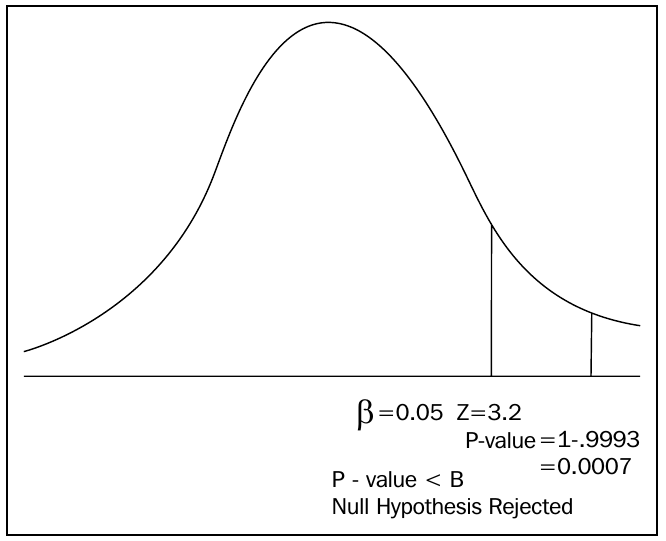
\includegraphics[height=5cm,keepaspectratio=true]{./images/kum0405.png}
	% kum0405.png: 0x0 pixel, 300dpi, 0.00x0.00 cm, bb=
	\caption{La hipótesis nula se rechaza porque el $p-$valor es menor al nivel de significación $\beta$.}
	\label{fig:0405}
\end{figure}

